\documentclass[11pt,a4paper]{article}

% ---------- Codificação e idioma ----------
\usepackage[utf8]{inputenc}
\usepackage[T1]{fontenc}
\usepackage[brazilian]{babel}
\usepackage{lmodern}
\usepackage{microtype}
\usepackage{amsmath}

% ---------- Layout ----------
\usepackage[a4paper, margin=2.3cm]{geometry}
\usepackage{setspace}
\onehalfspacing
\usepackage{parskip}

% ---------- Gráficos e tabelas ----------
\usepackage{graphicx}
\usepackage{caption}
\captionsetup{font=small,labelfont=bf,skip=4pt}
\usepackage{booktabs}
\usepackage{array}
\usepackage{tabularx}
\usepackage{multirow}
\usepackage{subcaption}
\usepackage{float}

% ---------- Cores / hyperref ----------
\usepackage{xcolor}
\definecolor{linkcol}{HTML}{0B4F8F}
\usepackage[colorlinks=true,
            linkcolor=linkcol,
            urlcolor=linkcol,
            citecolor=linkcol]{hyperref}

% ---------- Tipografia ----------
\usepackage{enumitem}
\setlist{itemsep=2pt,topsep=2pt}
\renewcommand{\arraystretch}{1.15}

% ---------- Cabeçalho e rodapé ----------
\usepackage{fancyhdr}
\pagestyle{fancy}
\fancyhf{}
\fancyhead[L]{\small INF01017 -- Aprendizado de Máquina}
\fancyhead[R]{\small T1 -- Car Evaluation}
\fancyfoot[C]{\thepage}
\renewcommand{\headrulewidth}{0.4pt}

% ---------- Atalhos ----------
\newcommand{\code}[1]{\texttt{\small #1}}

% =====================================================================
\begin{document}

% ---------- Cabeçalho ----------
\begin{center}
{\large\textbf{Universidade Federal do Rio Grande do Sul}}\\[2pt]
{\normalsize Instituto de Informática --- INF01017 Aprendizado de Máquina}\\[2pt]
{\normalsize Prof\textsuperscript{a}. Mariana Recamonde Mendoza}\\[16pt]

{\Large\bfseries Trabalho Prático Final --- Parte 1 (T1)}\\[6pt]
{\large\bfseries Coleta de dados, Análise Exploratória, Pré-processamento e Spot-checking \\
do conjunto \textit{Car Evaluation}}\\[8pt]
\end{center}

\vspace{4pt}

% \begin{center}

% \end{center}

\vspace{6pt}\hrule\vspace{12pt}

% =====================================================================
\section{Coleta de dados e identificação do problema}

\subsection{Origem e contexto do conjunto}
O conjunto \emph{Car Evaluation Database}, criado por Bohanec e Rajkovi\v{c} em 1988, foi derivado de um modelo hierárquico de decisão (DEX) construído originalmente para demonstrar sistemas especialistas multicritério. O conjunto está disponível publicamente no UCI Machine Learning Repository sob o identificador \textbf{19} e pode ser acessado em \url{https://archive.ics.uci.edu/dataset/19/car+evaluation}.

Por construção, o conjunto enumera \emph{todas} as combinações possíveis dos seis atributos preditores ($4 \cdot 4 \cdot 4 \cdot 3 \cdot 3 \cdot 3 = 1728$); a base não foi obtida por amostragem, mas sim pela aplicação determinística do modelo DEX a cada uma das 1.728 instâncias do espaço cartesiano de atributos.

\subsection{Pergunta de pesquisa e tarefa preditiva}
Pretende-se construir um modelo capaz de \textbf{prever a aceitabilidade global de um automóvel} a partir de seis características descritivas. Trata-se, portanto, de um problema de \textbf{classificação multiclasse} com quatro rótulos ordenados:
\begin{center}
\code{unacc} (inaceitável) $\prec$ \code{acc} (aceitável) $\prec$ \code{good} (bom) $\prec$ \code{vgood} (muito bom).
\end{center}

\subsection{Atributos do conjunto}
Os seis atributos preditores são todos categóricos, possuem ordem natural e baixa cardinalidade (Tabela~\ref{tab:atributos}). A classe possui também ordem natural, o que abre espaço para abordagens \emph{ordinais} de modelagem (avaliadas mais adiante).

\begin{table}[H]
\centering
\caption{Atributos preditores e respectivos domínios (ordem natural crescente).}
\label{tab:atributos}
\small
\begin{tabular}{lll c}
\toprule
\textbf{Atributo} & \textbf{Significado} & \textbf{Domínio (ordem natural $\rightarrow$)} & \textbf{Cardinalidade} \\
\midrule
\code{buying}   & preço de compra      & low, med, high, vhigh   & 4 \\
\code{maint}    & custo de manutenção  & low, med, high, vhigh   & 4 \\
\code{doors}    &   de portas     & 2, 3, 4, 5more          & 4 \\
\code{persons}  & capacidade           & 2, 4, more              & 3 \\
\code{lug\_boot} & porta-malas          & small, med, big         & 3 \\
\code{safety}   & segurança estimada   & low, med, high          & 3 \\
\bottomrule
\end{tabular}
\end{table}

\subsection{Justificativa da escolha do conjunto}
Foram consideradas as seguintes vantagens para a seleção:
\begin{itemize}
\item domínio de fácil interpretação, com atributos auto-explicativos;
\item tamanho moderado ($\approx$1,7k instâncias), compatível com a abordagem de \textit{spot-checking} prevista no T1;
\item ausência de valores faltantes e necessidade mínima de limpeza;
\item presença simultânea de classes desbalanceadas e atributos ordinais, o que permitirá discutir vieses indutivos diversos na fase posterior;
\item por ter sido gerado a partir de um modelo de regras hierárquicas conhecido, há expectativa de que algoritmos baseados em árvores recuperem boa parte da estrutura --- referência útil para comparar diferentes vieses indutivos.
\end{itemize}

% =====================================================================
\section{Análise exploratória dos dados}

\subsection{Inspeção inicial e qualidade dos dados}

A carga foi feita diretamente do arquivo \code{car.data}, atribuindo nomes às colunas conforme \code{car.names} e tipando cada atributo como \emph{categórico ordenado} respeitando sua ordem natural. A inspeção inicial revelou:

\begin{itemize}
\item \textbf{Dimensões:} 1.728 linhas $\times$ 7 colunas (6 atributos preditores + classe);
\item \textbf{Valores faltantes:} nenhum (\code{0/1728} em todas as colunas);
\item \textbf{Linhas duplicadas:} nenhuma --- coerente com o fato de o conjunto ser o produto cartesiano completo;
\item \textbf{Tipos:} todas as variáveis são categóricas; nenhum atributo numérico.
\end{itemize}

A combinação de dados sem ruído, completos e sem duplicatas indica que \textbf{não há demandas de imputação ou remoção} de instâncias.

\subsection{Distribuição do atributo alvo}

A Figura~\ref{fig:target} apresenta a distribuição da variável \code{class}. A base é \textbf{fortemente desbalanceada}: aproximadamente 70\,\% das instâncias correspondem à classe \code{unacc}, enquanto as classes \code{good} e \code{vgood} somam menos de 8\,\%. A razão entre a classe majoritária e a minoritária é de aproximadamente $1210/65 \approx 18{,}6\times$.

\begin{figure}[H]
\centering
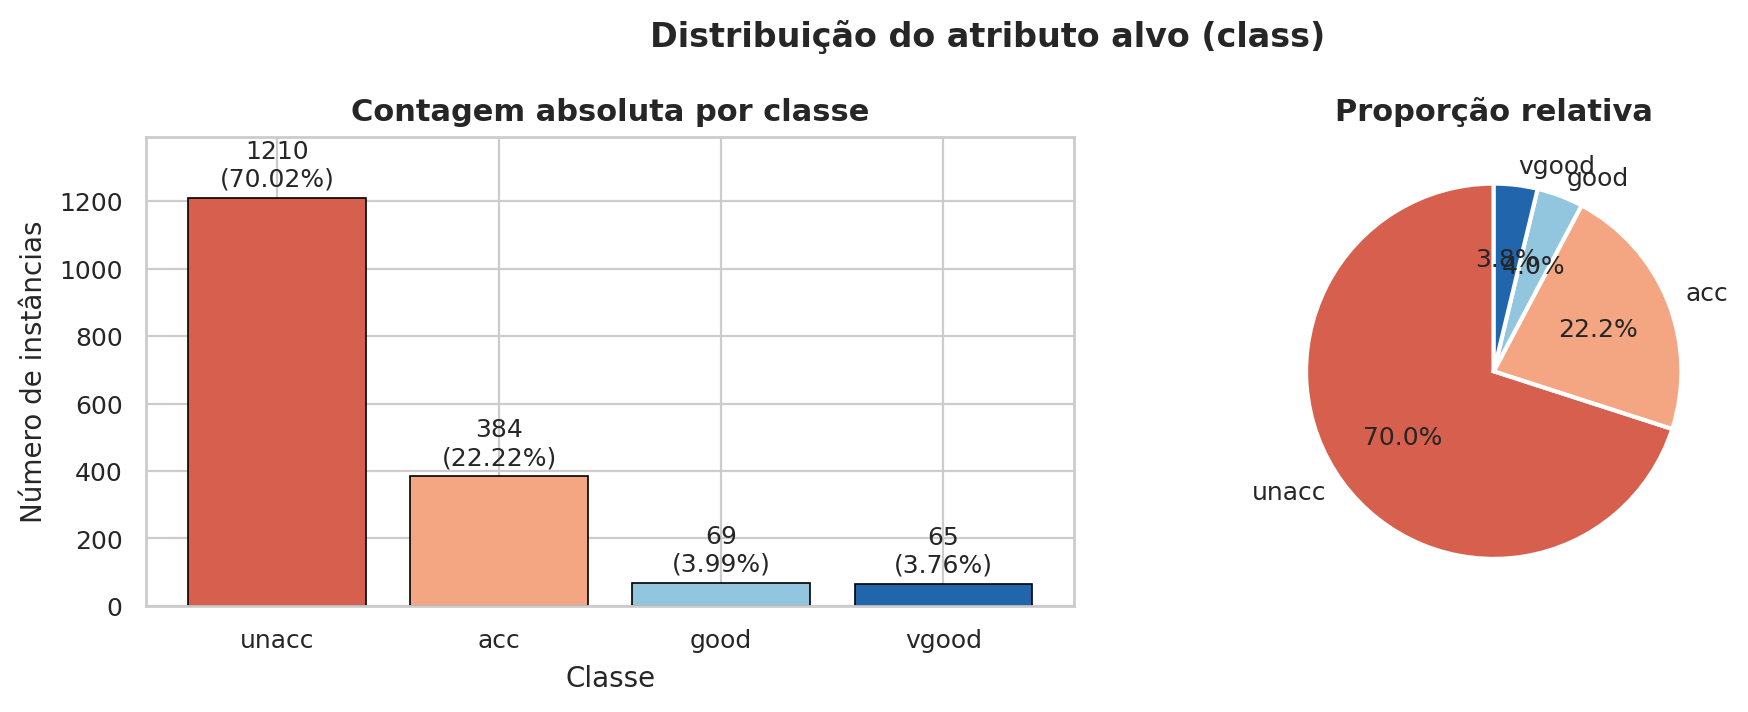
\includegraphics[width=0.95\textwidth]{figures/01_target_distribution.png}
\caption{Distribuição do atributo alvo \code{class}. À esquerda, contagens absolutas; à direita, proporções relativas.}
\label{fig:target}
\end{figure}

\textbf{Implicações.} O desbalanceamento severo torna a acurácia simples uma métrica enganosa: um classificador trivial que sempre prediga \code{unacc} já alcançaria $\approx$70\,\% de acerto. Em consequência, recomenda-se na fase de \textit{spot-checking}:
\begin{itemize}
\item \textbf{métrica principal:} F1 macro ou \textit{balanced accuracy};
\item \textbf{métricas secundárias:} F1 por classe, matriz de confusão, acurácia;
\item \textbf{validação cruzada estratificada}, para preservar as proporções (especialmente das classes minoritárias \code{good} e \code{vgood}).
\end{itemize}

\subsection{Distribuição dos atributos preditores}

A Figura~\ref{fig:features} mostra que \textbf{todos os atributos têm distribuição marginal exatamente uniforme}: 432 instâncias por valor para os atributos com cardinalidade 4 e 576 instâncias por valor para os atributos com cardinalidade 3.

\begin{figure}[H]
\centering
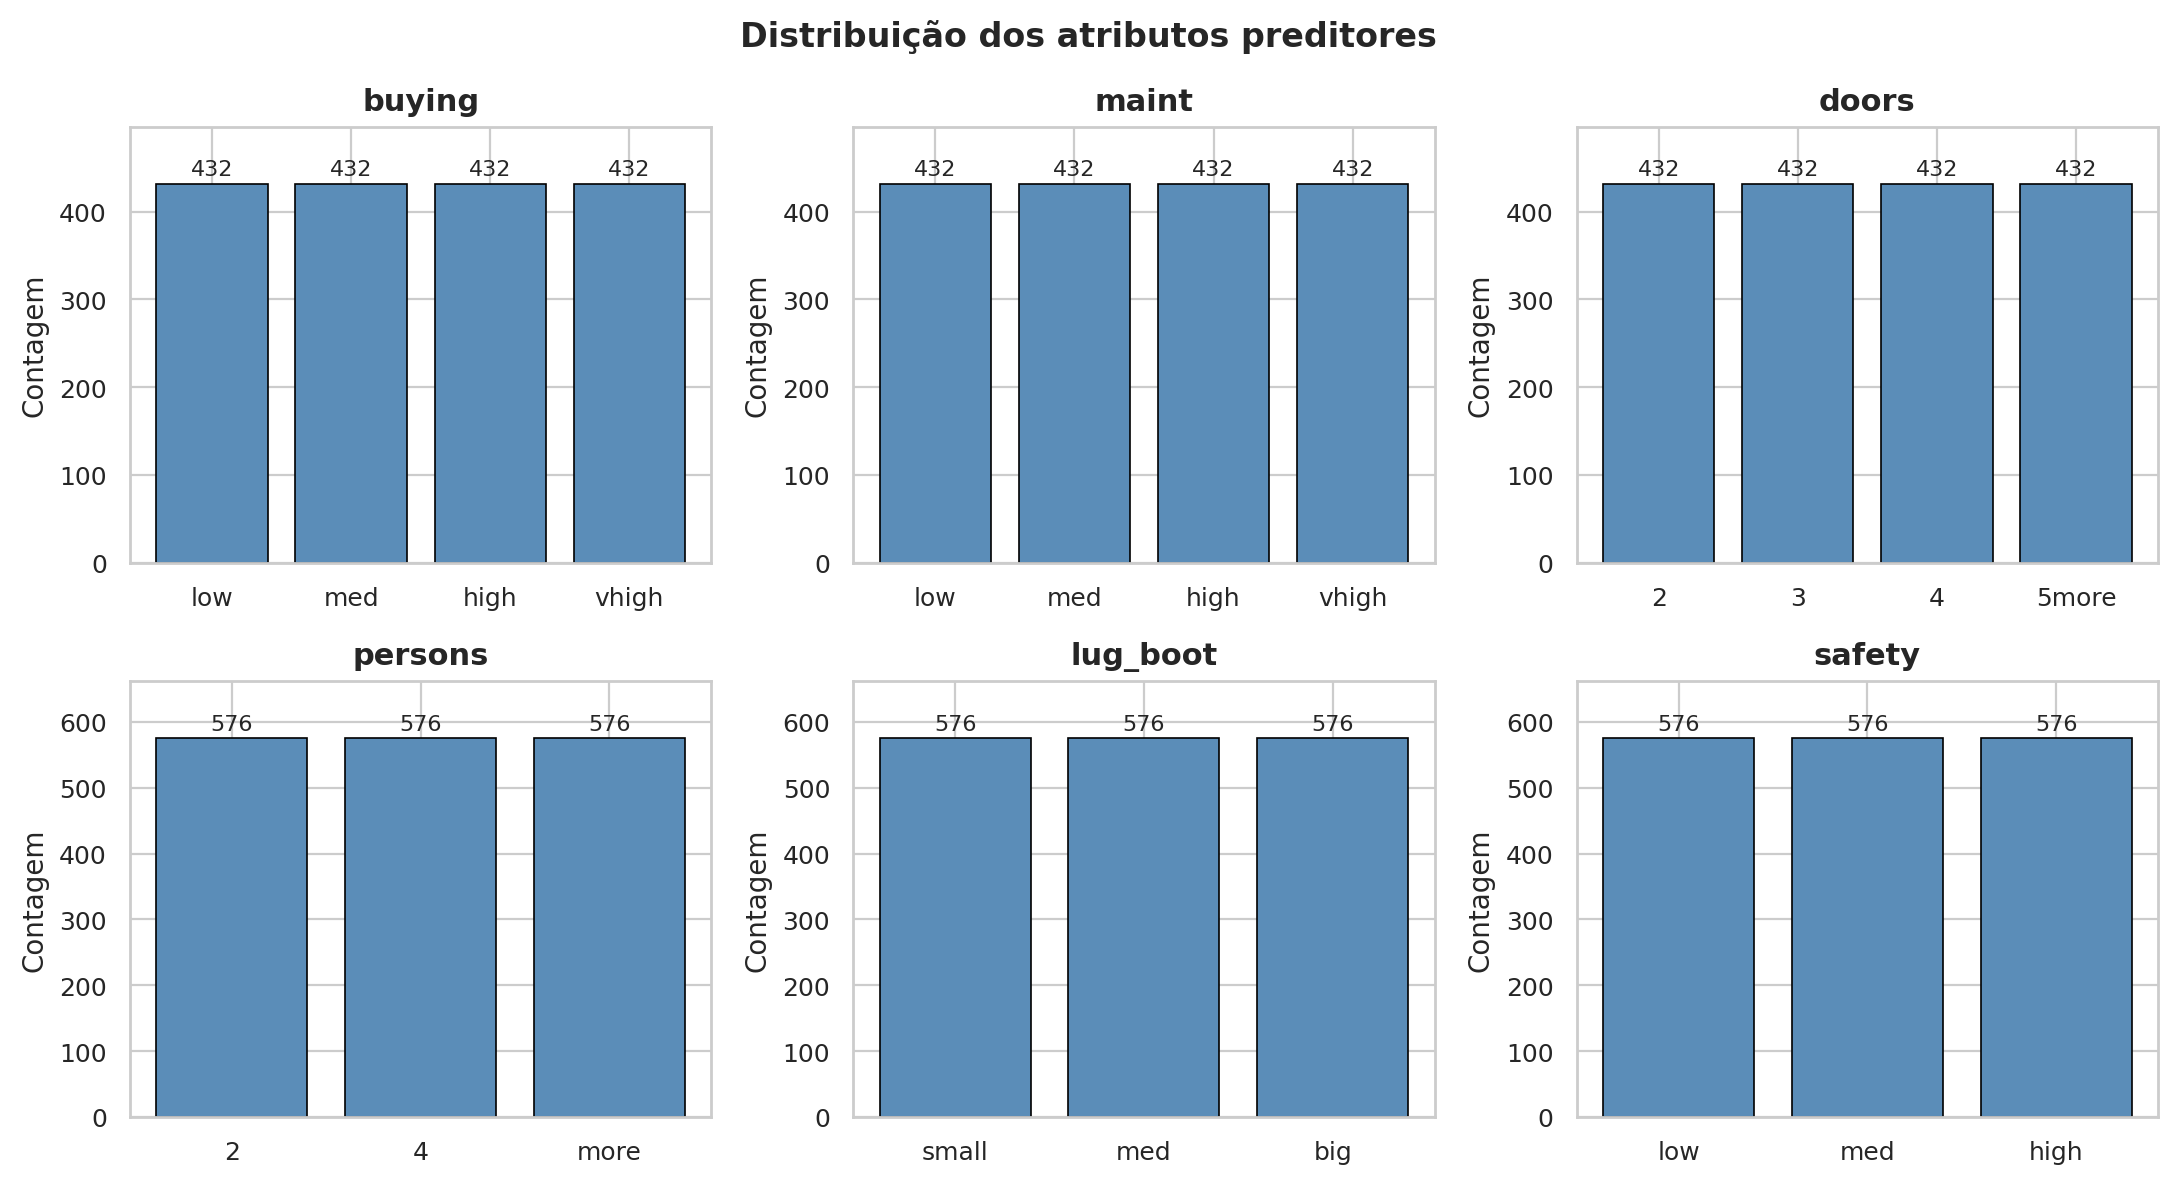
\includegraphics[width=0.92\textwidth]{figures/02_features_distribution.png}
\caption{Distribuição marginal de cada atributo preditor. A uniformidade perfeita decorre da construção do conjunto como produto cartesiano dos domínios.}
\label{fig:features}
\end{figure}

\subsection{Análise bivariada: classe condicionada ao atributo}

A Figura~\ref{fig:bivar} apresenta, para cada atributo, a distribuição da classe entre os valores do atributo (proporções normalizadas por linha).

\begin{figure}[H]
\centering
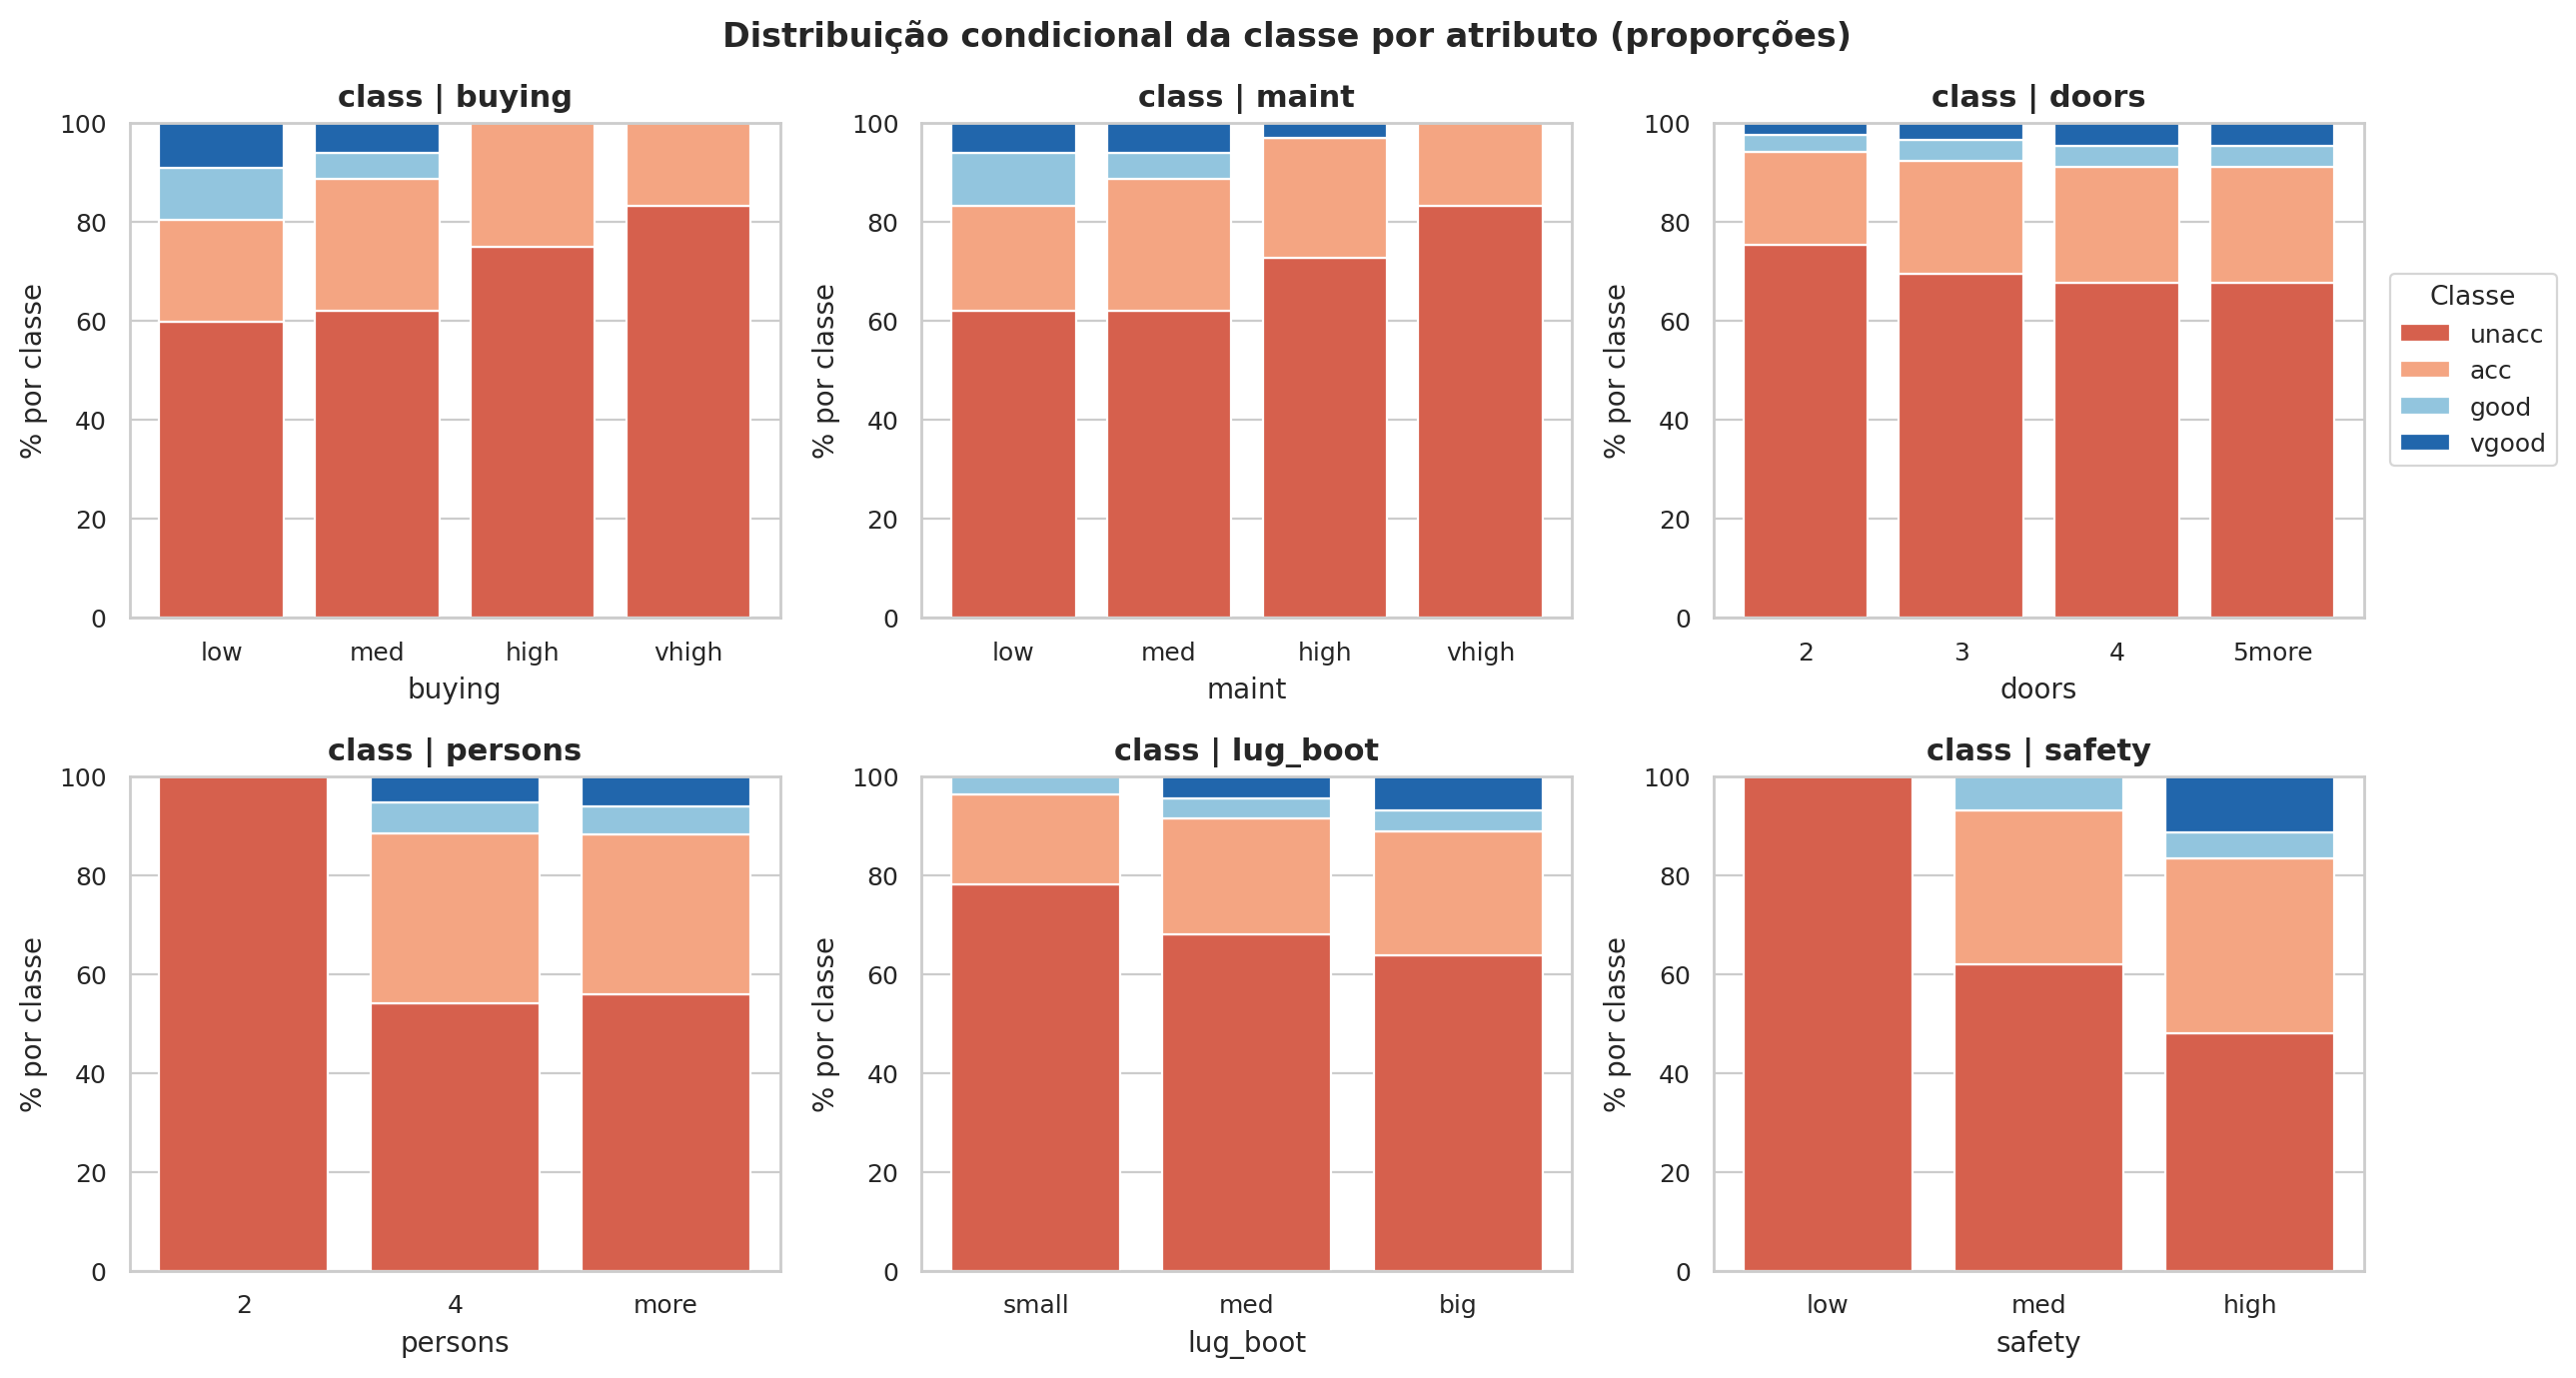
\includegraphics[width=\textwidth]{figures/03_class_by_feature.png}
\caption{Distribuição condicional $P(\mathrm{classe} \mid \mathrm{atributo})$ para cada um dos seis atributos preditores.}
\label{fig:bivar}
\end{figure}

\noindent Vários padrões saltam aos olhos:

\begin{itemize}
\item \textbf{Regras determinísticas:} \code{safety = low} $\Rightarrow$ 100\,\% \code{unacc} (576/576) e \code{persons = 2} $\Rightarrow$ 100\,\% \code{unacc} (576/576). Estas duas regras isoladas já explicam $960/1210 \approx 79\%$ das instâncias inaceitáveis, e correspondem a restrições de bom senso (carro sem segurança ou apenas dois lugares dificilmente atende a uma família).
\item \textbf{Restrição em \code{lug\_boot}:} a classe \code{vgood} \emph{nunca} ocorre quando \code{lug\_boot = small} ($P=0$).
\item \textbf{Tendências monotônicas:} \code{buying} e \code{maint} apresentam aumento monotônico em $P(\code{unacc})$ à medida que o preço/manutenção sobem; \code{persons}, \code{lug\_boot} e \code{safety} mostram comportamento contrário (aumentar o atributo melhora a avaliação).
\item \textbf{Atributo aparentemente irrelevante:} \code{doors} produz distribuições praticamente idênticas em todos os seus quatro níveis.
\end{itemize}

\subsection{Heatmap de probabilidades condicionais}

Para reforçar visualmente os padrões discutidos, a Figura~\ref{fig:heatmap} apresenta as matrizes $P(\code{class} \mid \text{atributo})$ na forma de \textit{heatmap}, com os atributos em ordem natural crescente.

\begin{figure}[H]
\centering
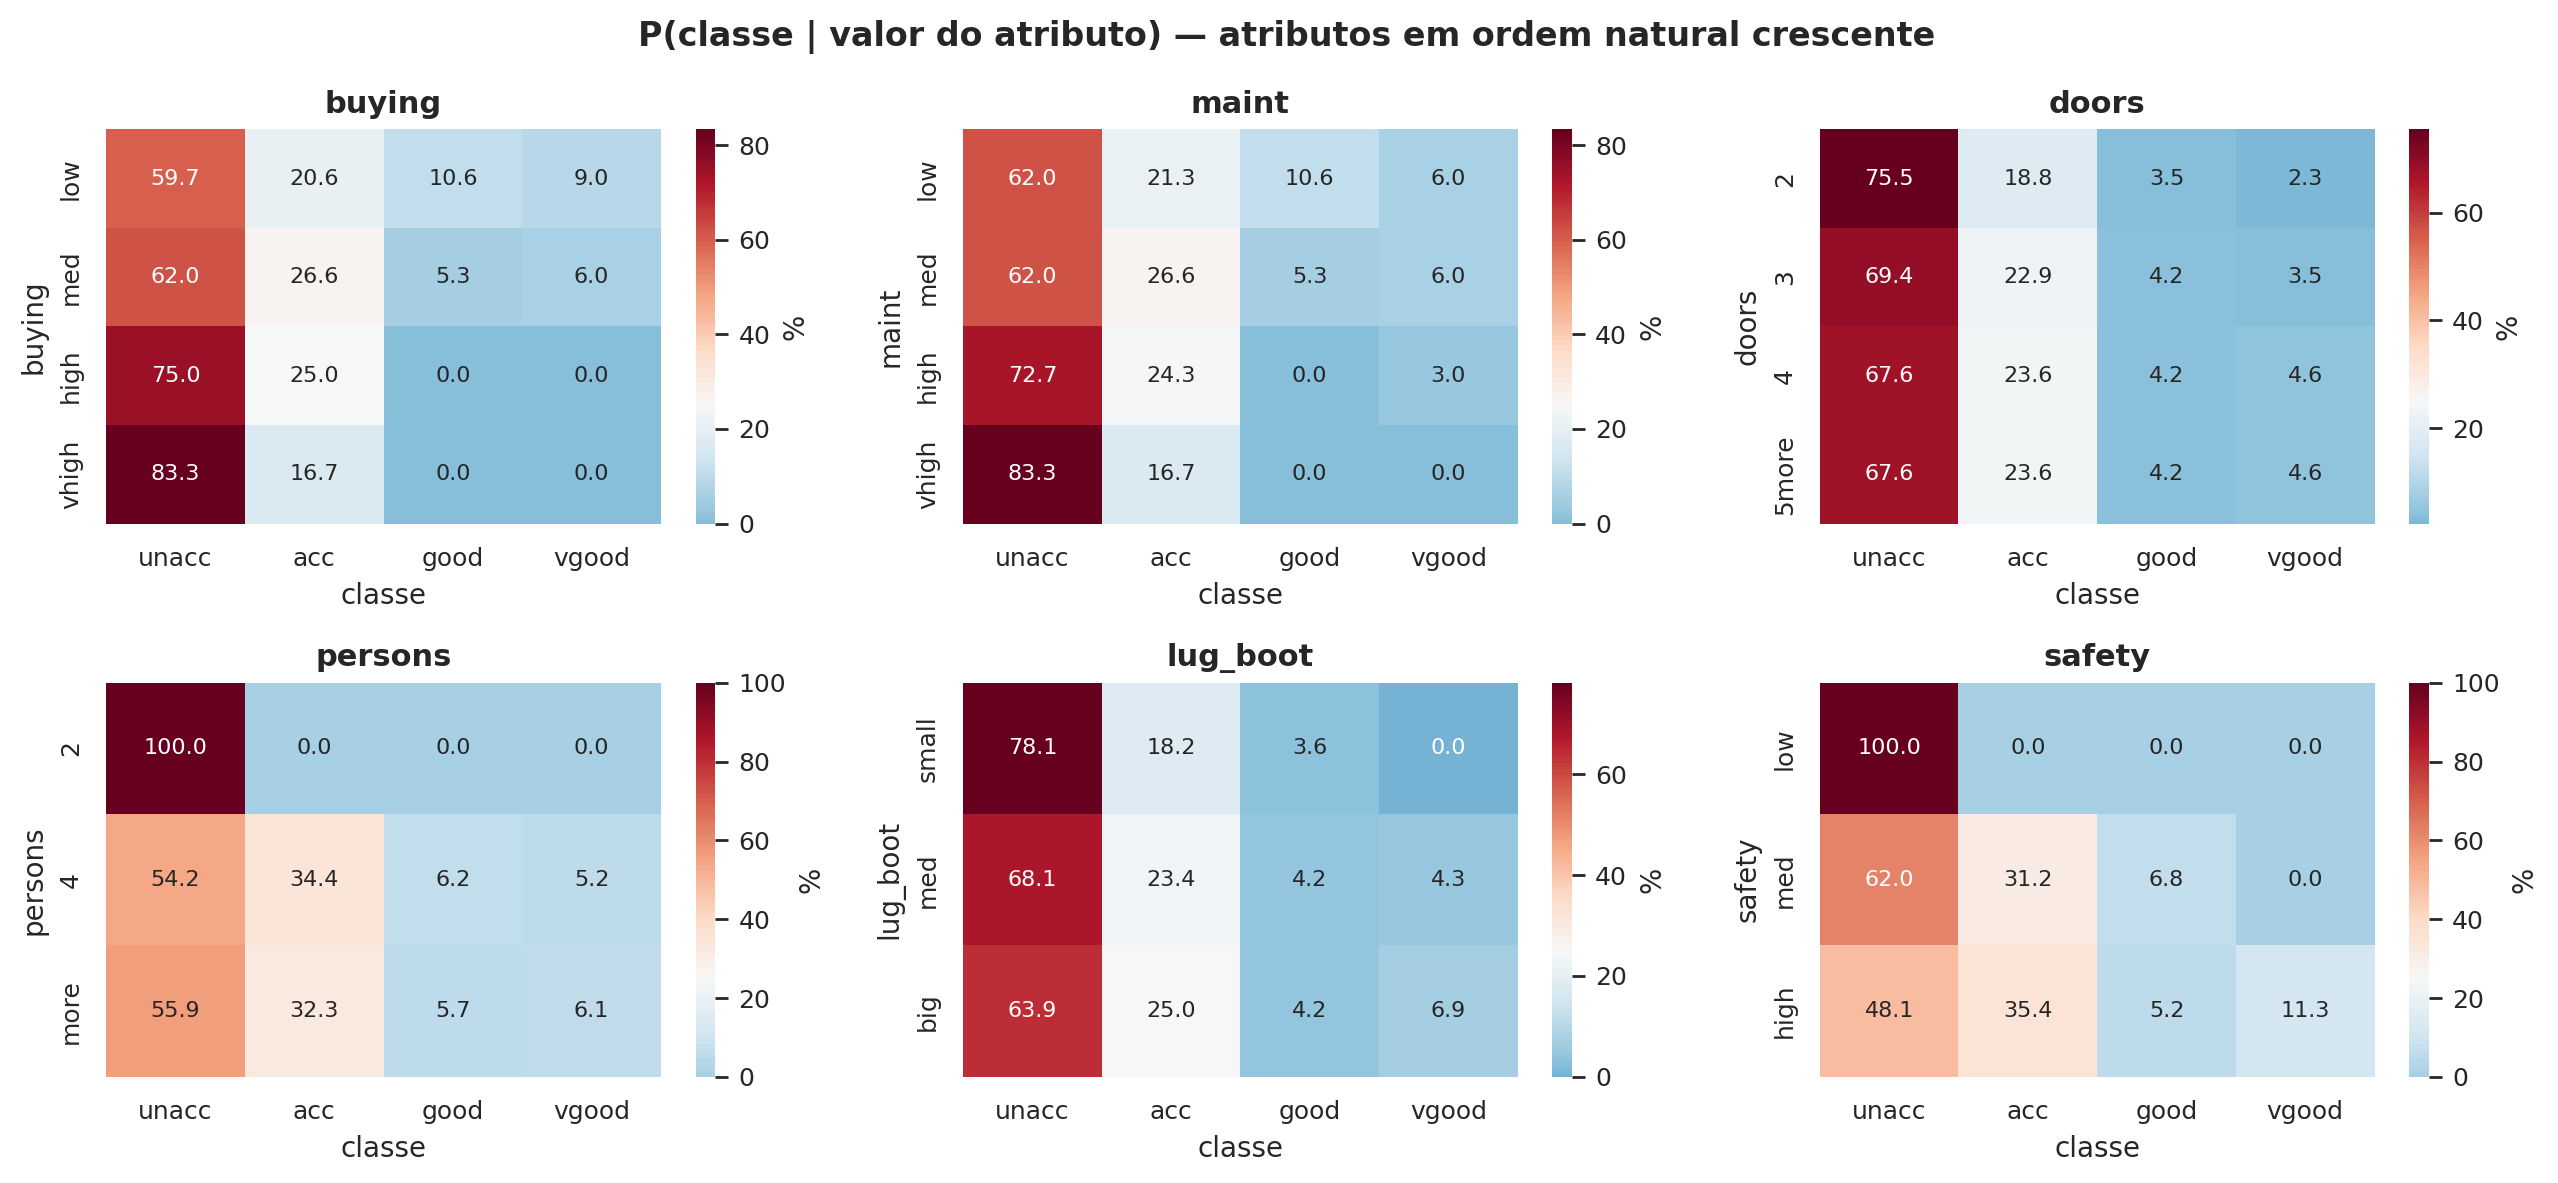
\includegraphics[width=\textwidth]{figures/04_monotonicity_heatmap.png}
\caption{Probabilidade da classe condicionada ao valor de cada atributo. Tons mais escuros indicam maior concentração; as linhas dos atributos estão ordenadas em ordem natural crescente, evidenciando os gradientes de monotonicidade discutidos.}
\label{fig:heatmap}
\end{figure}

% =====================================================================
\section{Conclusões da análise exploratória}
\label{sec:conclusoes_EDA}
A análise permitiu uma caracterização completa do conjunto e fornece direcionamento concreto para a próxima etapa do trabalho.

\paragraph{Características do conjunto.}
\begin{enumerate}
\item Tamanho de 1.728 instâncias e seis atributos preditores categóricos ordinais, gerados como produto cartesiano completo --- portanto sem aleatoriedade na construção;
\item qualidade dos dados é excelente: nenhum valor faltante, nenhuma duplicata, nenhum \textit{outlier} categórico --- todos os atributos têm distribuição marginal exatamente uniforme;
\item o problema é de \textbf{classificação multiclasse com classes ordenadas} e fortemente desbalanceadas (razão majoritária/minoritária de $\approx 18{,}6\times$).
\end{enumerate}

\paragraph{Regras determinísticas observadas.}
\begin{enumerate}
\setcounter{enumi}{3}
\item \code{safety = low} $\Rightarrow$ 100\,\% \code{unacc} (576/576);
\item \code{persons = 2} $\Rightarrow$ 100\,\% \code{unacc} (576/576);
\item \code{lug\_boot = small} $\Rightarrow$ nunca classifica como \code{vgood}.
\end{enumerate}

\paragraph{Implicações para o \textit{spot-checking}.}
\begin{itemize}
\item \textbf{Métrica principal:} F1 macro (ou \textit{balanced accuracy}), em razão do desbalanceamento severo;
\item \textbf{Métricas secundárias:} acurácia, F1 por classe e matriz de confusão;
\item \textbf{Validação:} \textit{stratified k-fold} para preservar proporções;
\end{itemize}

\paragraph{Necessidades de pré-processamento.}
A EDA aponta as seguintes ações como pertinentes para a fase posterior do trabalho:
\begin{itemize}
\item codificação dos atributos categóricos --- duas alternativas a se considerar: \emph{ordinal} (preserva a ordem natural identificada) e \emph{one-hot} (trata como nominal);
\item tratamento do desbalanceamento (no mínimo, estratificação na validação cruzada);
\item avaliar manter ou descartar \code{doors}, dado que as distribuições de classe são praticamente idênticas em todos os seus quatro níveis.
\end{itemize}
\section{Treinamento do modelo}
\noindent
\subsection{Algoritmos e Métricas de desempenho}
\begin{minipage}[t]{0.45\textwidth}
\textbf{Algoritmos utilizados:}
\begin{itemize}
    \item K-nearest neighbors
    \item Regressão Logística
    \item Árvore de decisão
    \item Rede Neural
    \item Naive Bayes
    \item SVM
    \item Florestas Aleatórias
    \item AdaBoost
\end{itemize}
\end{minipage}
\hfill
\begin{minipage}[t]{0.45\textwidth}
\textbf{Métricas utilizadas}
\begin{itemize}
    \item Acurácia
    \item Acurácia balanceada
    \item Recall
    \item Precisão
    \item F1-Micro
    \item F1-Macro
    \item ROC-AUC
\end{itemize}
\end{minipage}
\subsection{Scores obtidos para cada algoritmo}
\begin{figure}[H]
    \centering
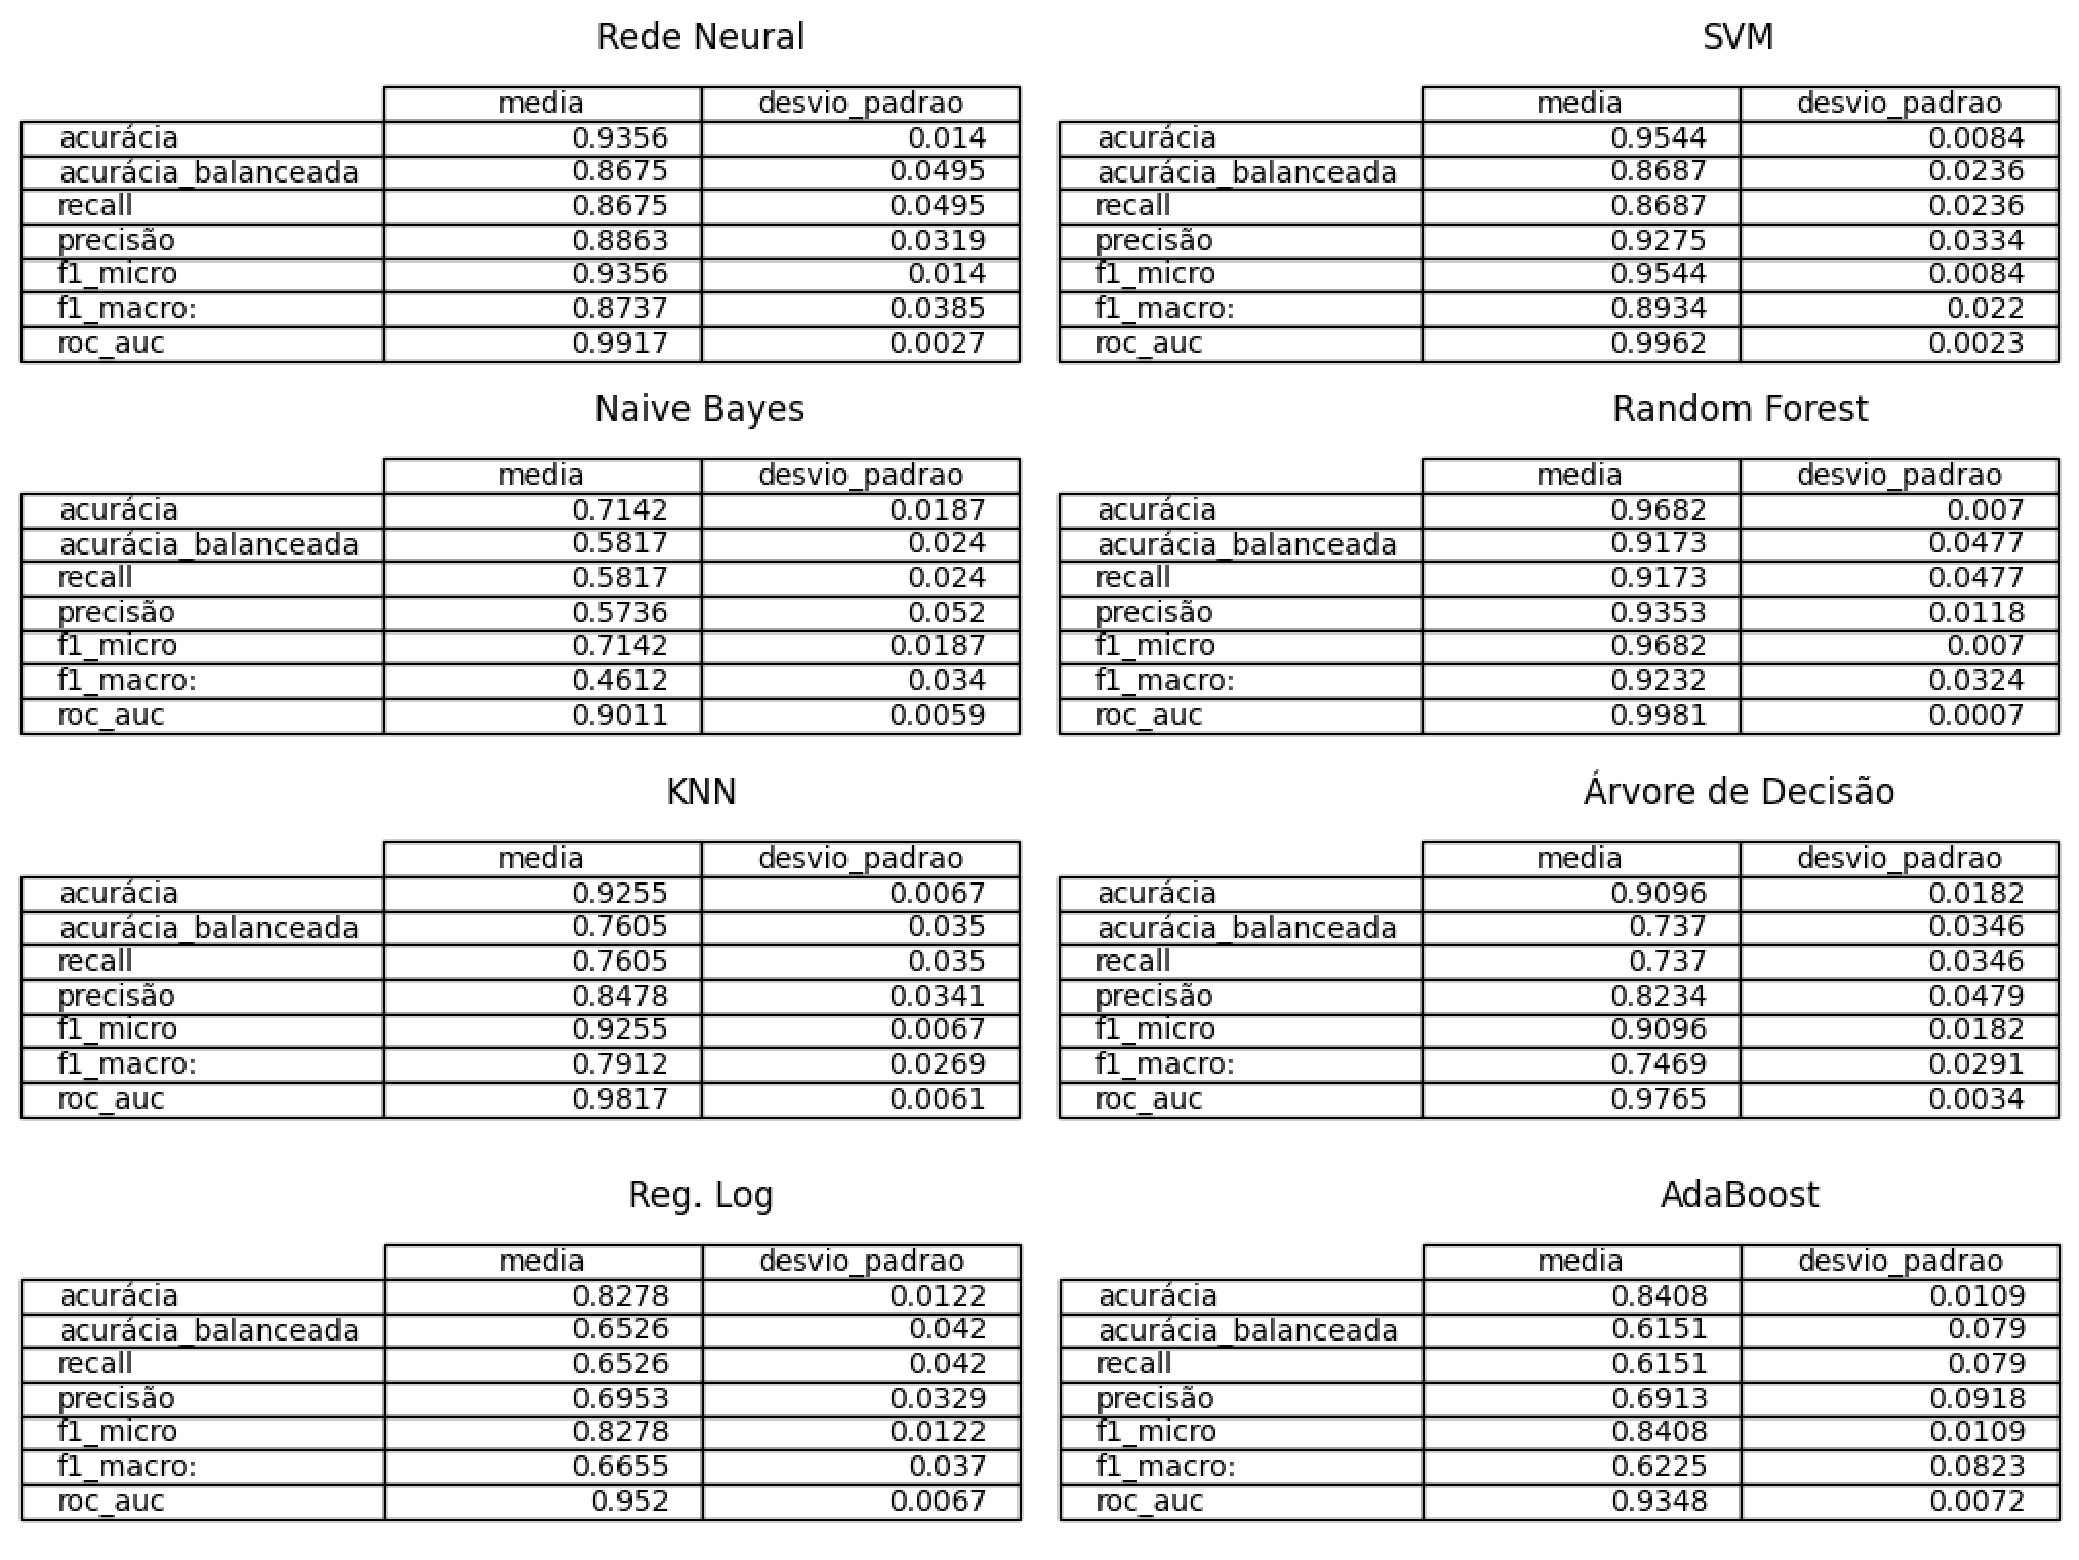
\includegraphics[width=\textwidth]{figures/05_score_tables.png}
    \caption{Score de cada algoritmo nas métricas utilizadas}
    \label{fig:placeholder}
\end{figure}
\subsection{Boxplot de cada métrica}
\begin{figure}[H]
    \centering
    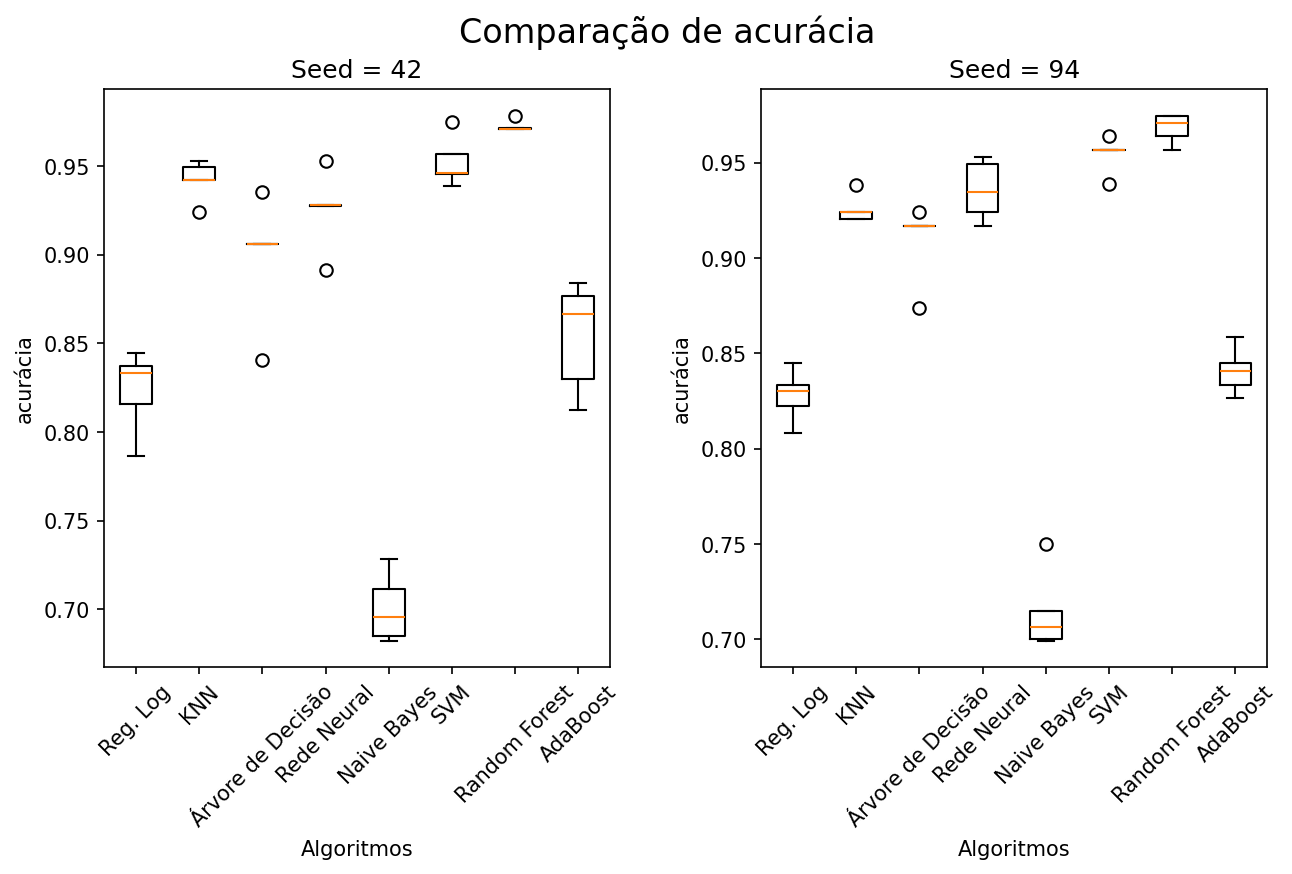
\includegraphics[width=0.8\textwidth]{figures/boxplots/06-boxplot_acc.png}
    \caption{Boxplot da acurácia}
\end{figure}

\begin{figure}[H]
    \centering
    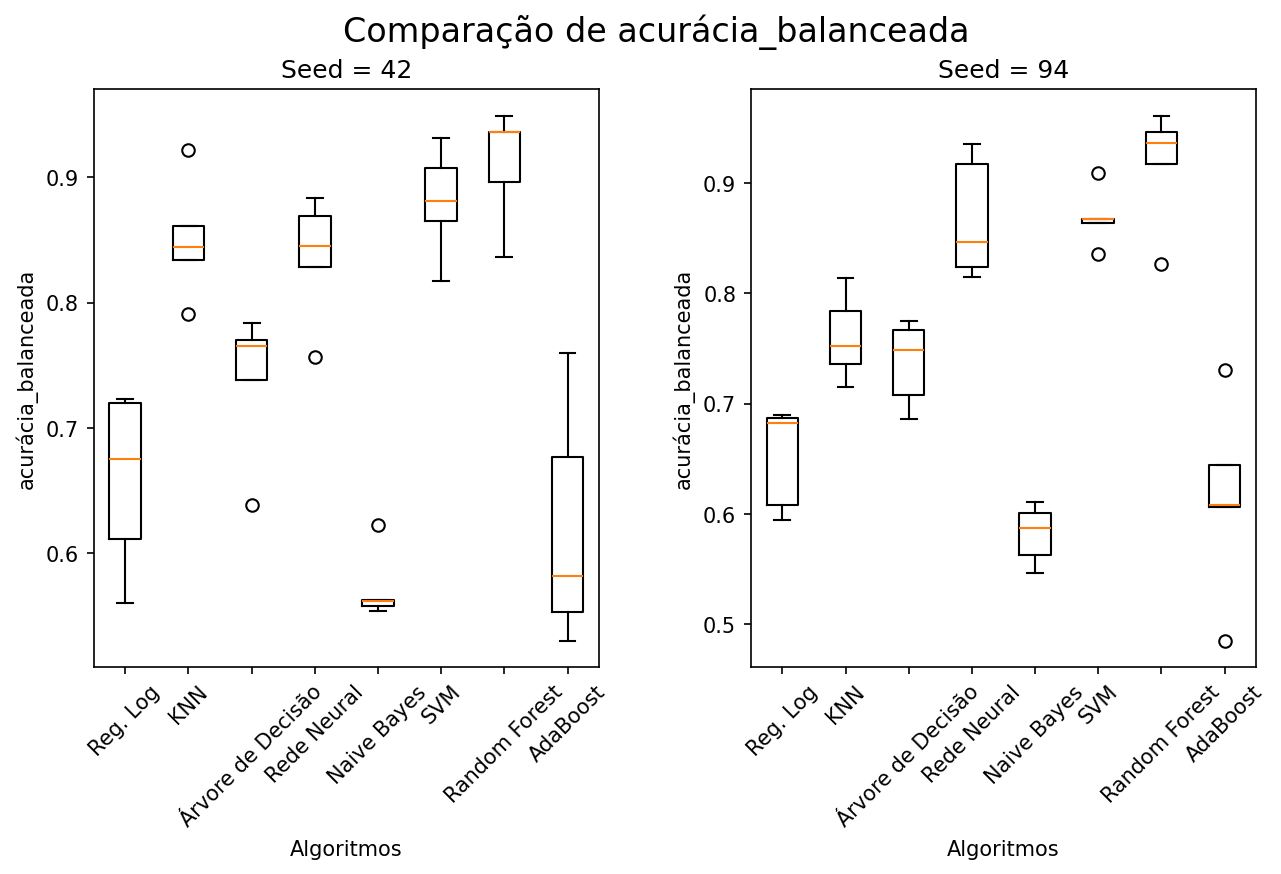
\includegraphics[width=0.8\textwidth]{figures/boxplots/07-boxplot_balanced_acc.png}
    \caption{Boxplot da acurácia balanceada}
\end{figure}

\begin{figure}[H]
    \centering
    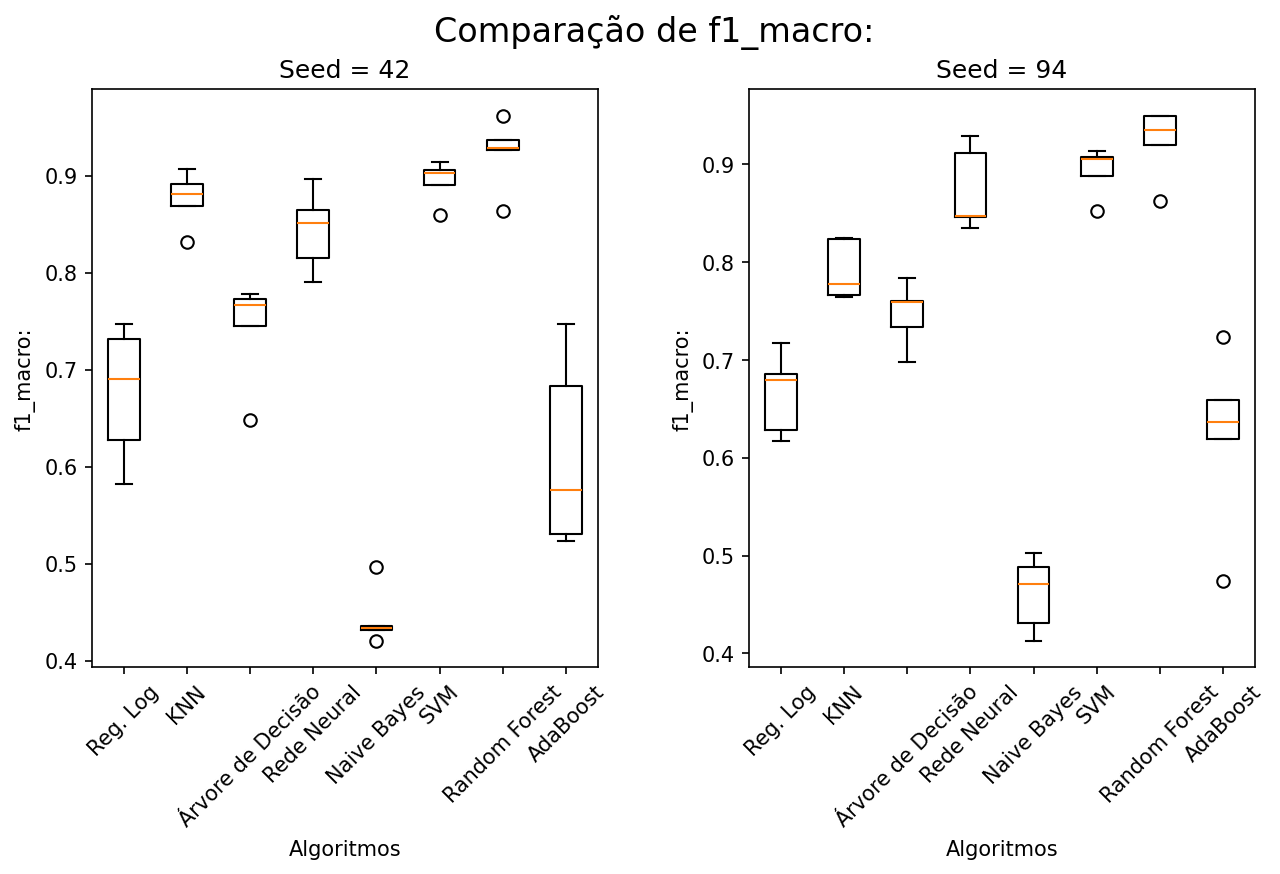
\includegraphics[width=0.8\textwidth]{figures/boxplots/08-boxplot_f1_macro.png}
    \caption{Boxplot do F1-Macro}
\end{figure}

\begin{figure}[H]
    \centering
    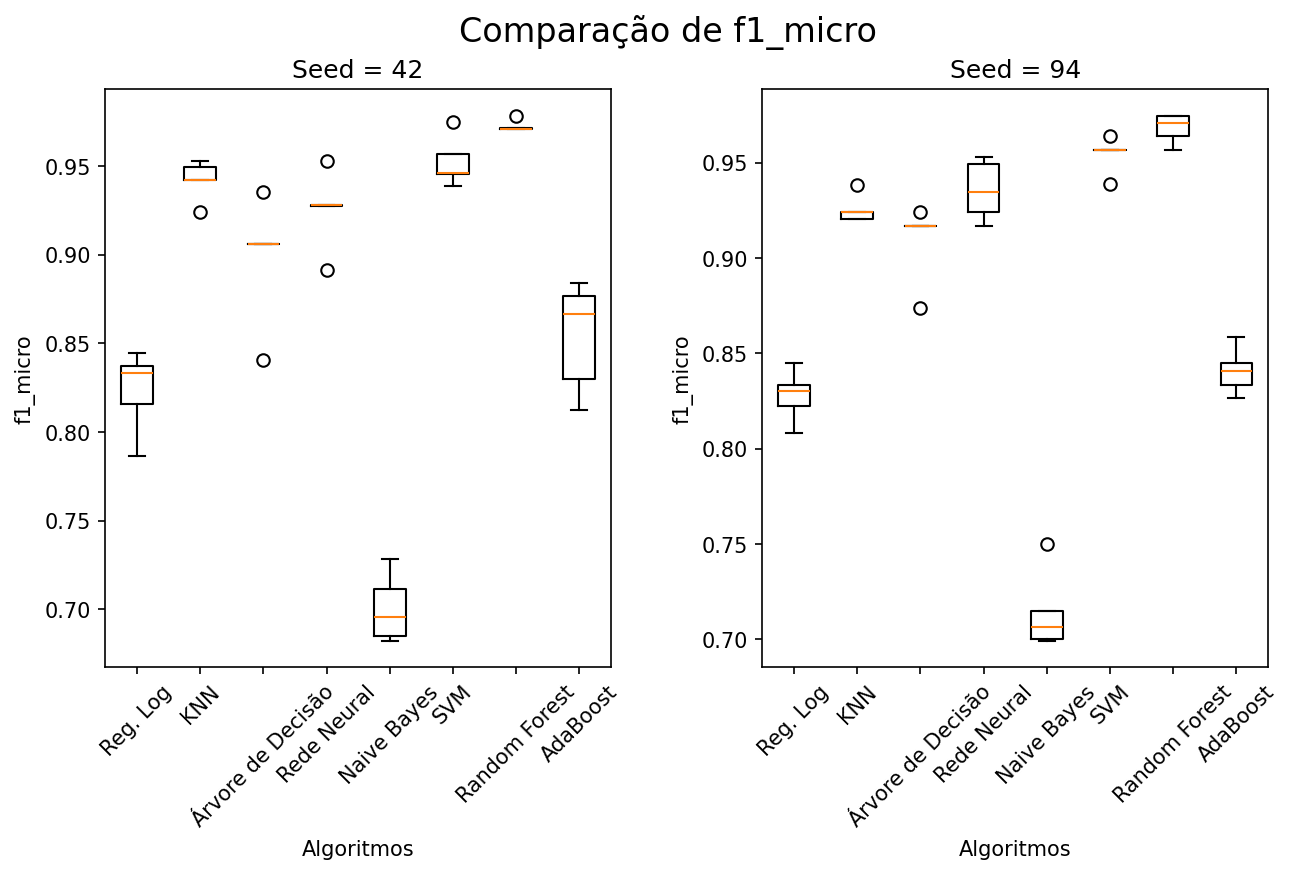
\includegraphics[width=0.8\textwidth]{figures/boxplots/09-boxplot_f1_micro.png}
    \caption{Boxplot do F1-Micro}
\end{figure}

\begin{figure}[H]
    \centering
    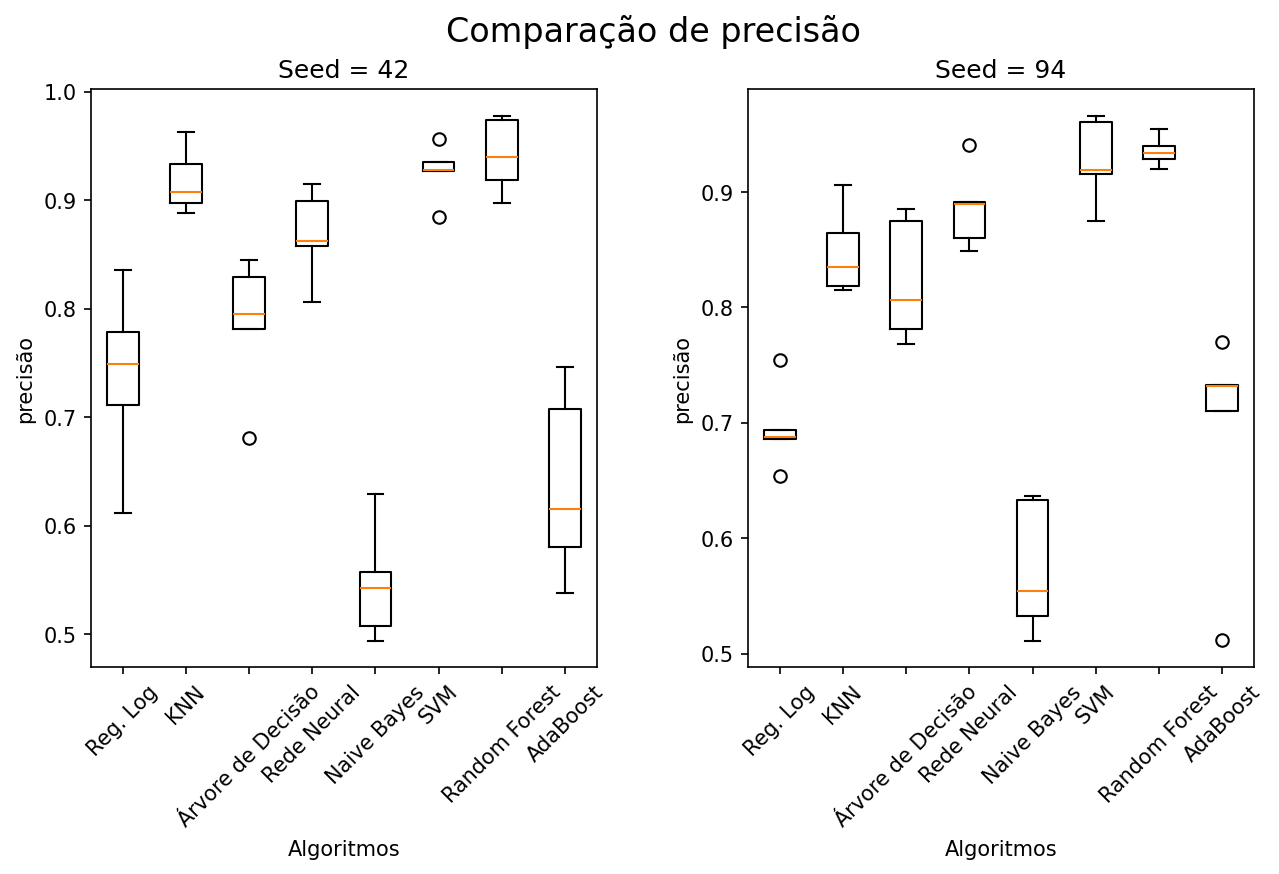
\includegraphics[width=0.8\textwidth]{figures/boxplots/10-boxplot_precision.png}
    \caption{Boxplot da precisão}
\end{figure}

\begin{figure}[H]
    \centering
    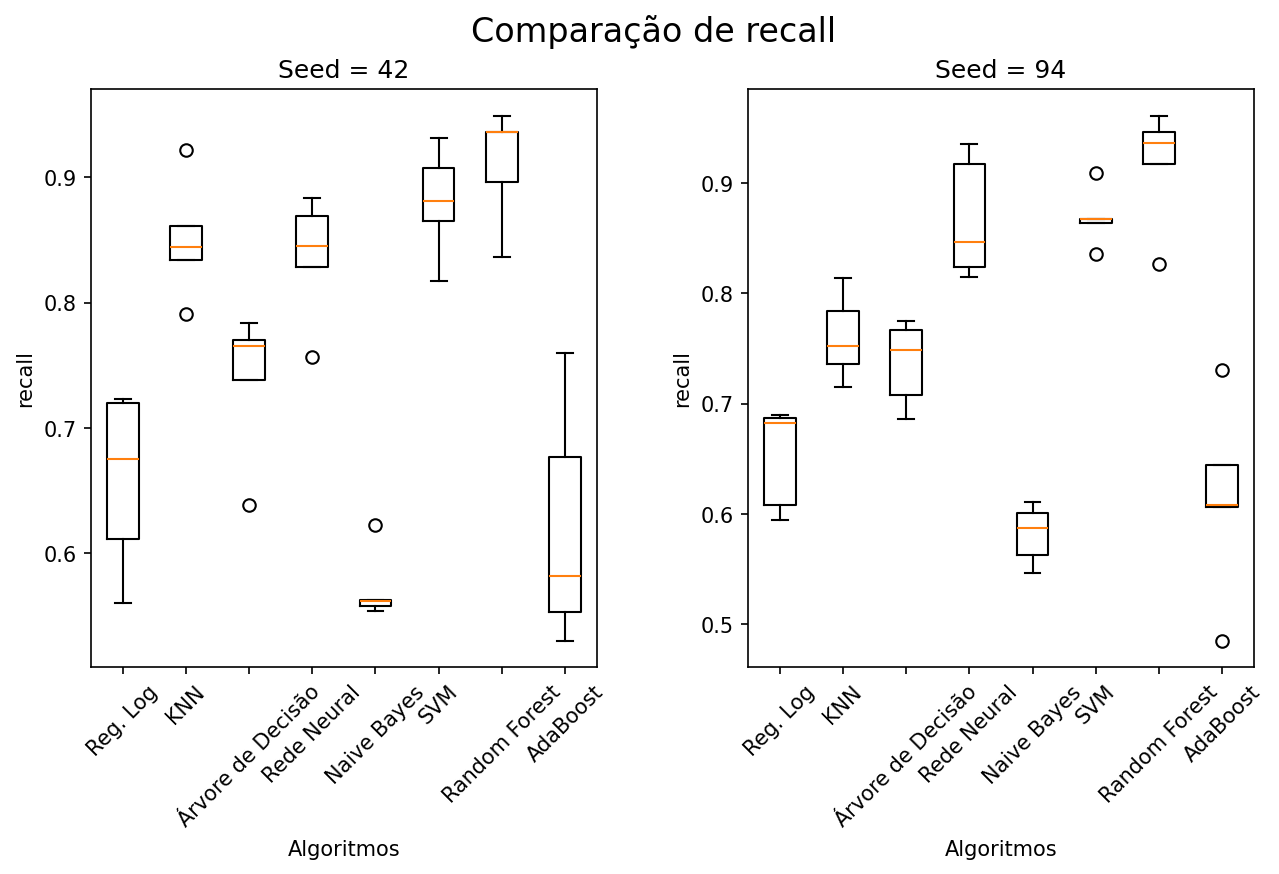
\includegraphics[width=0.8\textwidth]{figures/boxplots/11-boxplot_recall.png}
    \caption{Boxplot do recall}
\end{figure}

\begin{figure}[H]
    \centering
    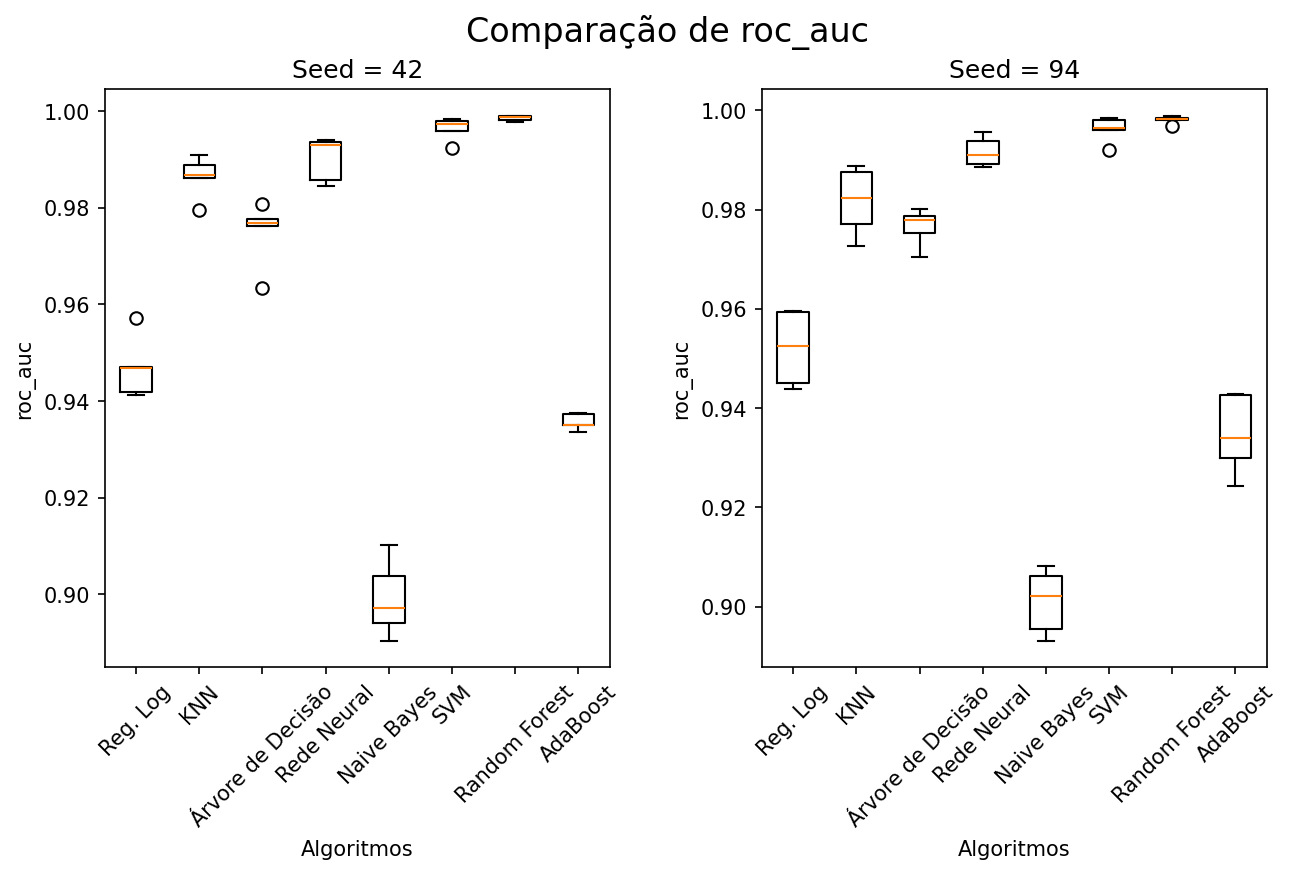
\includegraphics[width=\textwidth]{figures/boxplots/12-boxplot_roc_aux.png}
    \caption{Boxplot do ROC-AUC}
\end{figure}

\subsection{Matriz de confusão dos algoritmos analisados}

\begin{figure}[H]
    \centering
    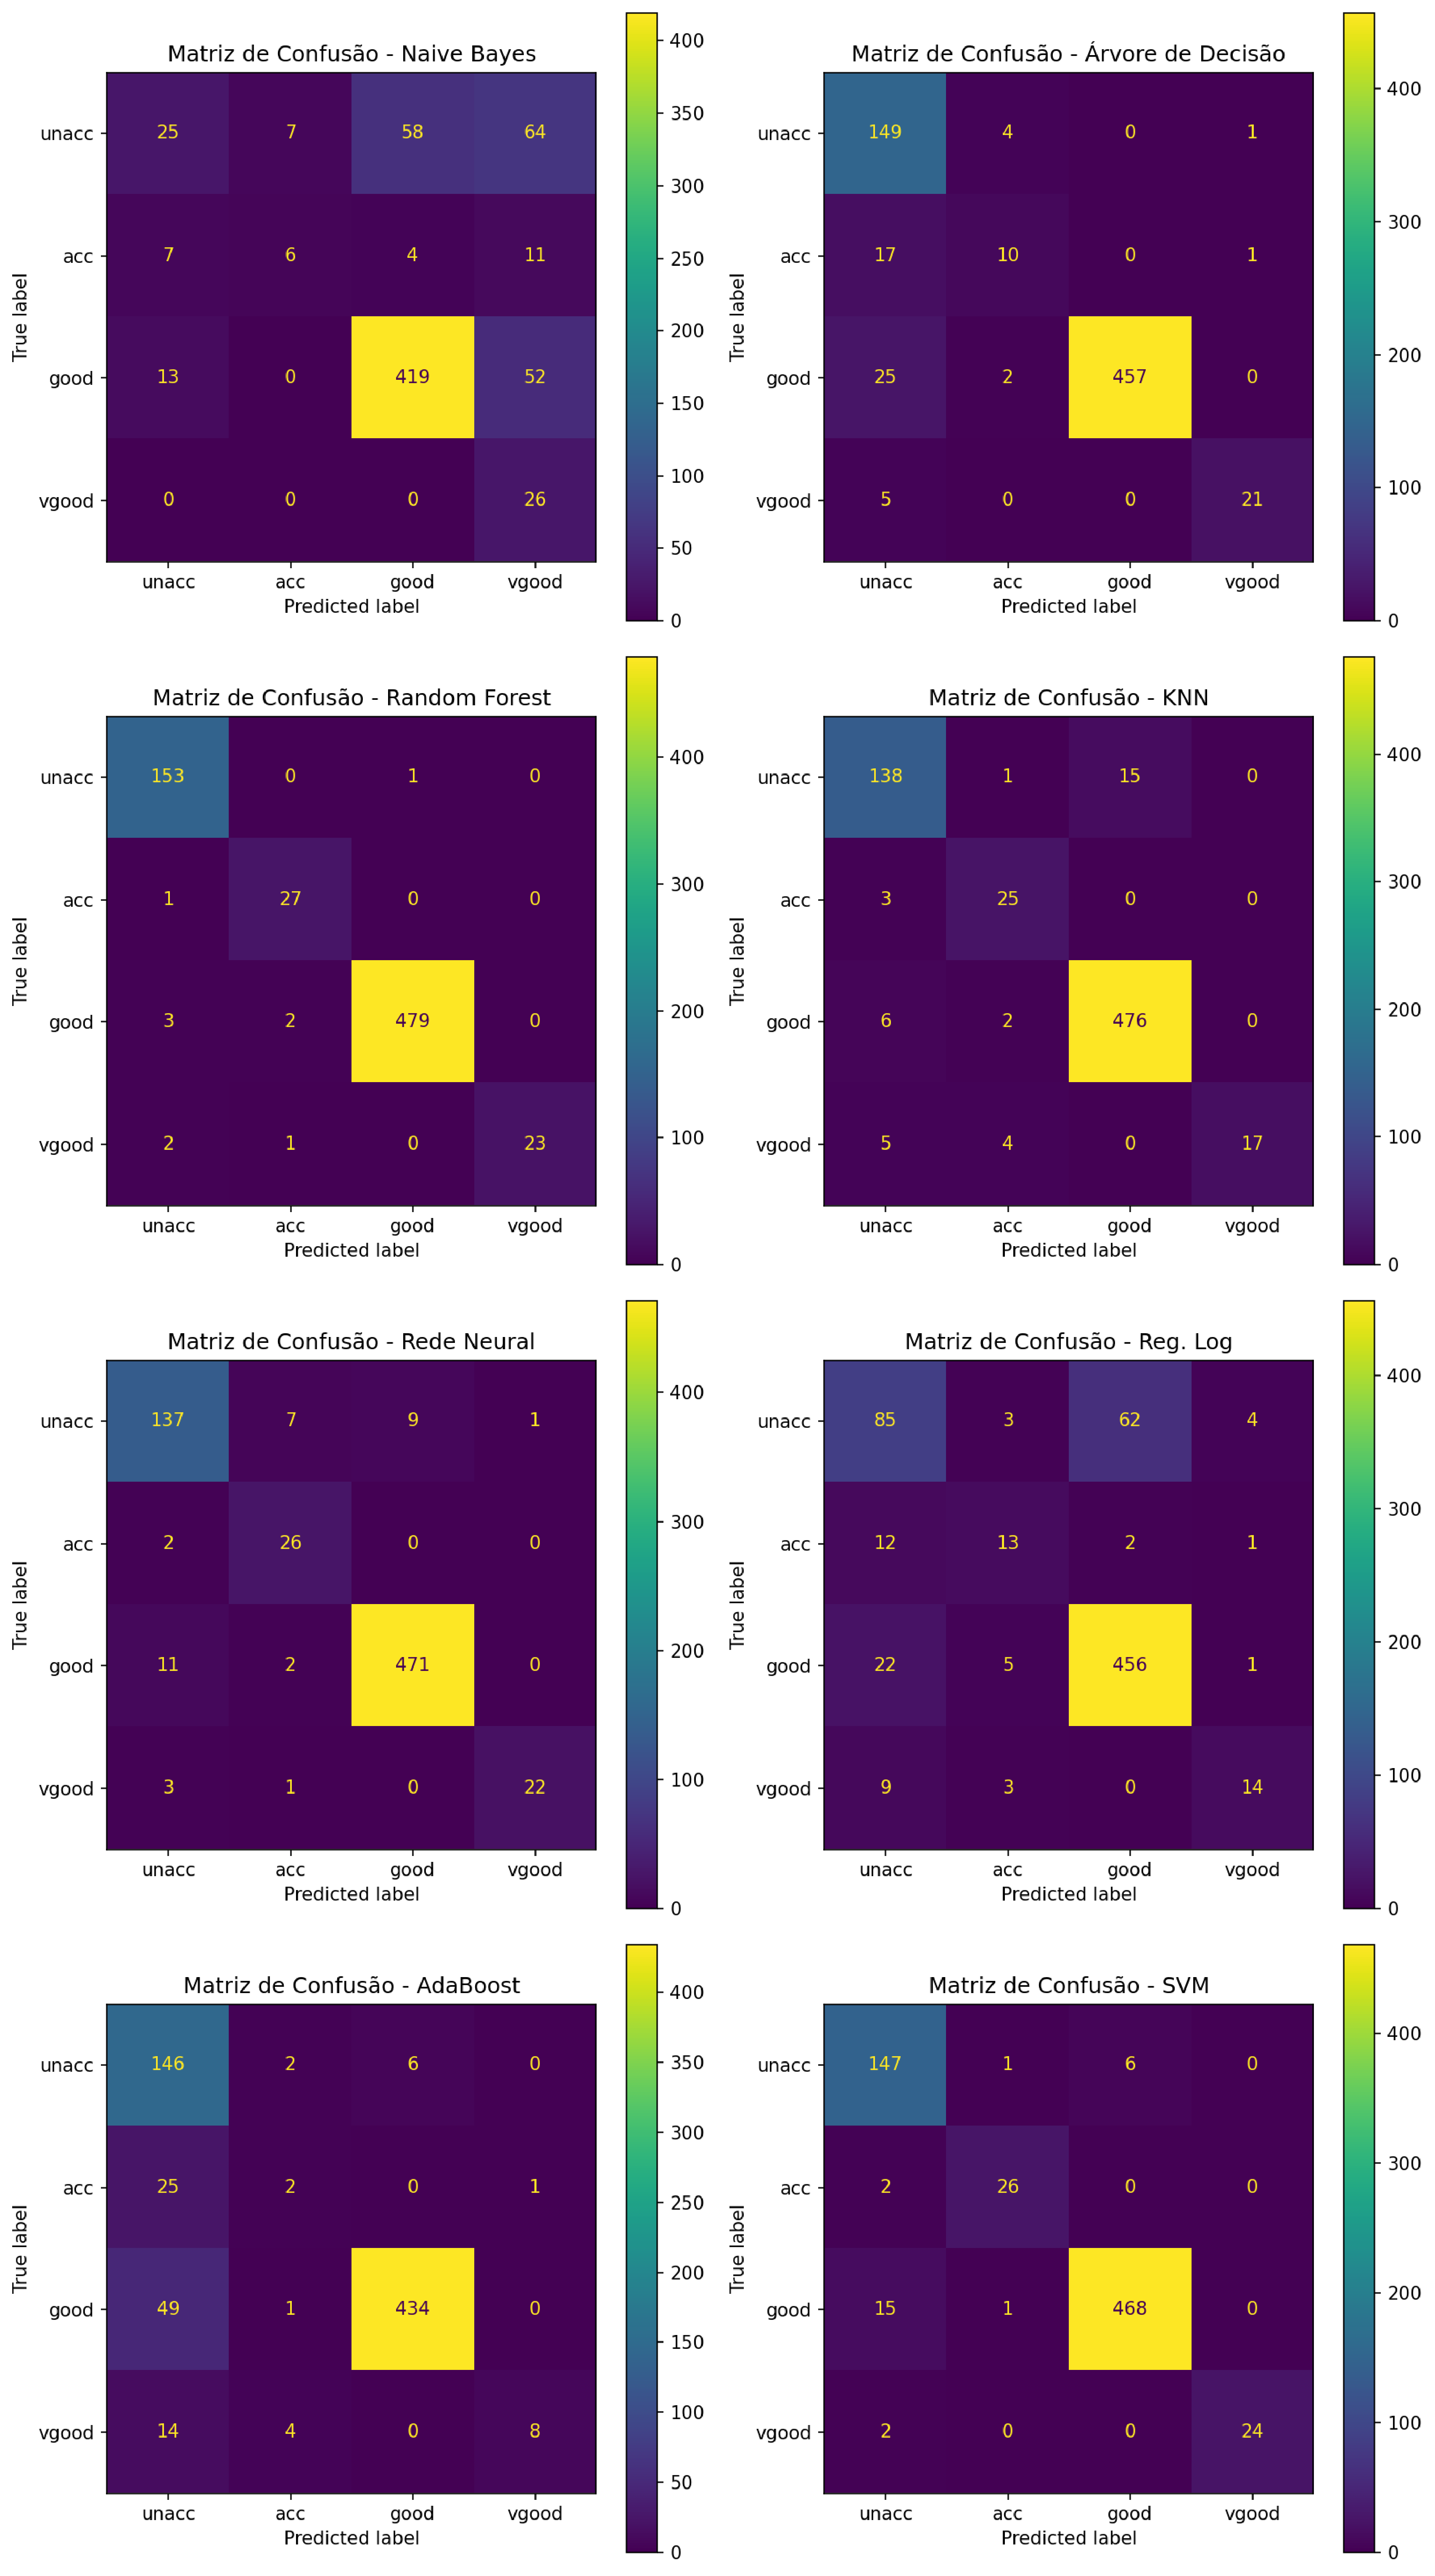
\includegraphics[width=0.6\linewidth]{figures/13_confusion_matrixes.pdf}
    \caption{Matriz de confusão para cada algoritmo avaliado}
    \label{fig:placeholder}
\end{figure}
\subsection{Conclusões sobre os algoritmos avaliados}
Considerando as métricas analisadas, o algoritmo que apresentou melhor desempenho foi o algoritmo de Florestas Aleatórias, com o F1-macro tendo um score de 0.9232 e uma acurácia balanceada de 0.9173. Devemos considerar essas duas métricas com mais rigor devido à natureza dos dados serem desbalanceadas, como visto na seção ~\ref{sec:conclusoes_EDA}. Entretanto, é interessante observar o comportamento coerente entre as métricas utilizadas e a natureza dos dados, onde todas as métricas utilizadas para dados balanceados se mostram elevadas de forma otimista. Também podemos observar através da matriz de confusão que o modelo se adaptou muito bem para  a predição de classes positivas, tendo apenas um desempenho inferior para classificar carros como acc (acceptable).
% =====================================================================
\begin{thebibliography}{9}

\bibitem{bohanec1988}
Bohanec, M. \& Rajkovi\v{c}, V. (1988).
\textit{Knowledge acquisition and explanation for multi-attribute decision making.}
8th Intl. Workshop on Expert Systems and their Applications, Avignon, France, pp. 59--78.

\bibitem{uci}
Dua, D. \& Graff, C. (2019).
\textit{UCI Machine Learning Repository.} University of California, Irvine.\\
\url{https://archive.ics.uci.edu/dataset/19/car+evaluation}

\bibitem{sklearn}
Pedregosa, F. et al. (2011).
\textit{Scikit-learn: Machine Learning in Python.}
Journal of Machine Learning Research, 12, 2825--2830.

\bibitem{faceli}
Faceli, K., Lorena, A. C., Gama, J. \& Carvalho, A. C. P. L. F. (2021).
\textit{Inteligência Artificial: Uma Abordagem de Aprendizado de Máquina} (2\textsuperscript{a} ed.).
LTC.

\end{thebibliography}

\end{document}
